\section{Anexos}

\begin{ilustracion}[ht]
    \centering
    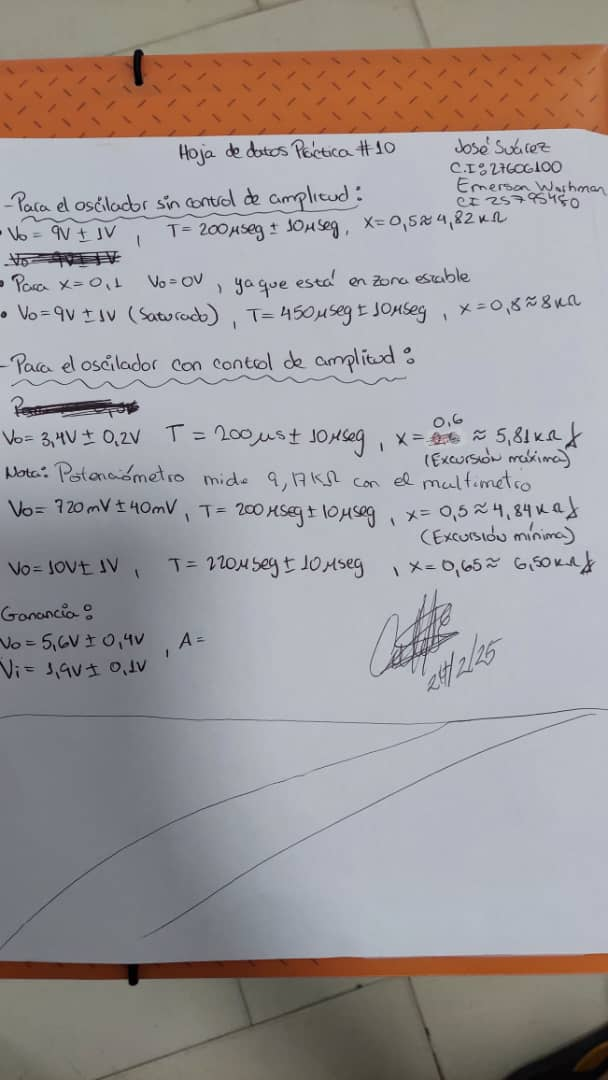
\includegraphics[width=0.9\textwidth]{hoja-de-datos-1.jpg}
    \caption{Hoja de datos práctica N° 6}
    \label{ilus:hoja-de-datos-1}
\end{ilustracion}

\begin{ilustracion}[ht]
    \centering
    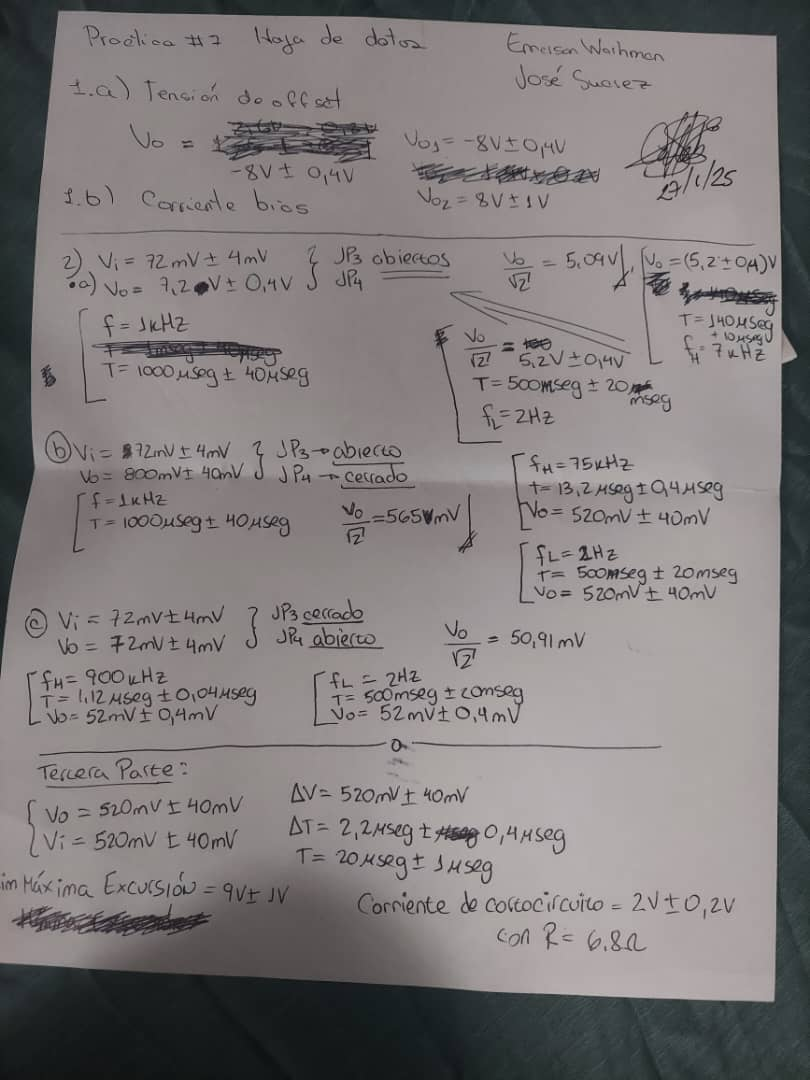
\includegraphics[width=0.9\textwidth]{hoja-de-datos-2.jpg}
    \caption{Hoja de datos práctica N° 7}
    \label{ilus:hoja-de-datos-2}
\end{ilustracion}

\begin{ilustracion}[ht]
    \centering
    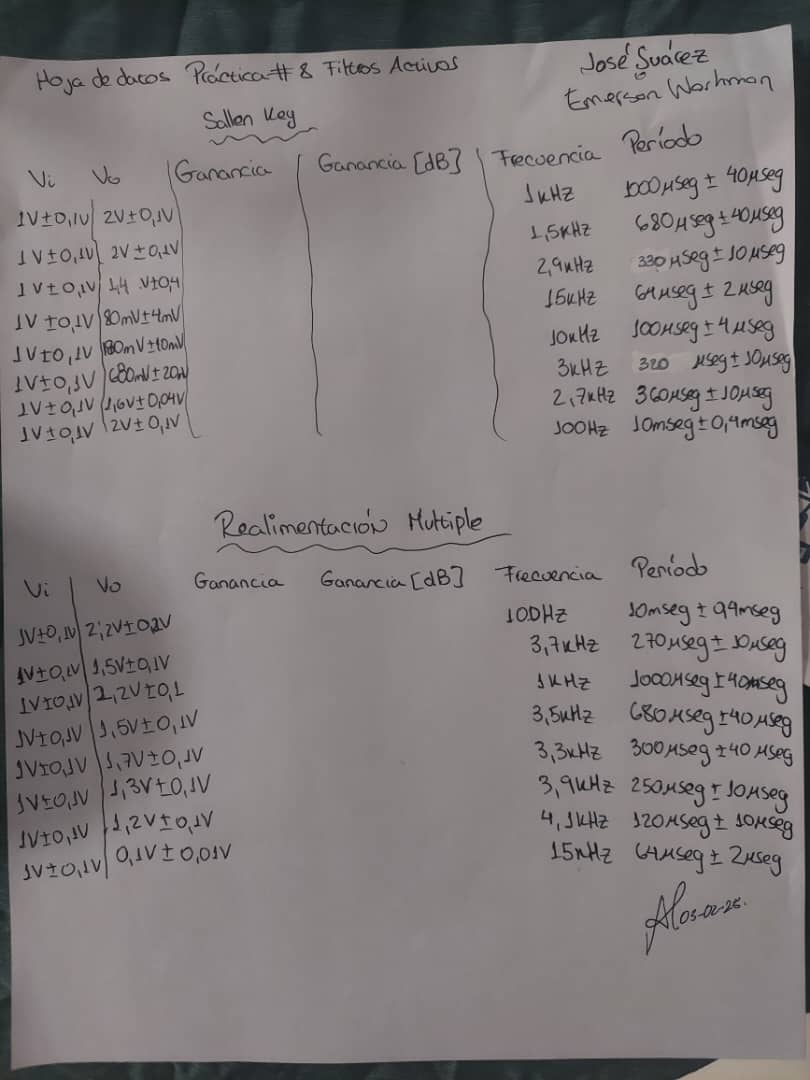
\includegraphics[width=0.9\textwidth]{hoja-de-datos-3.png}
    \caption{Hoja de datos práctica N° 8}
    \label{ilus:hoja-de-datos-3}
\end{ilustracion}



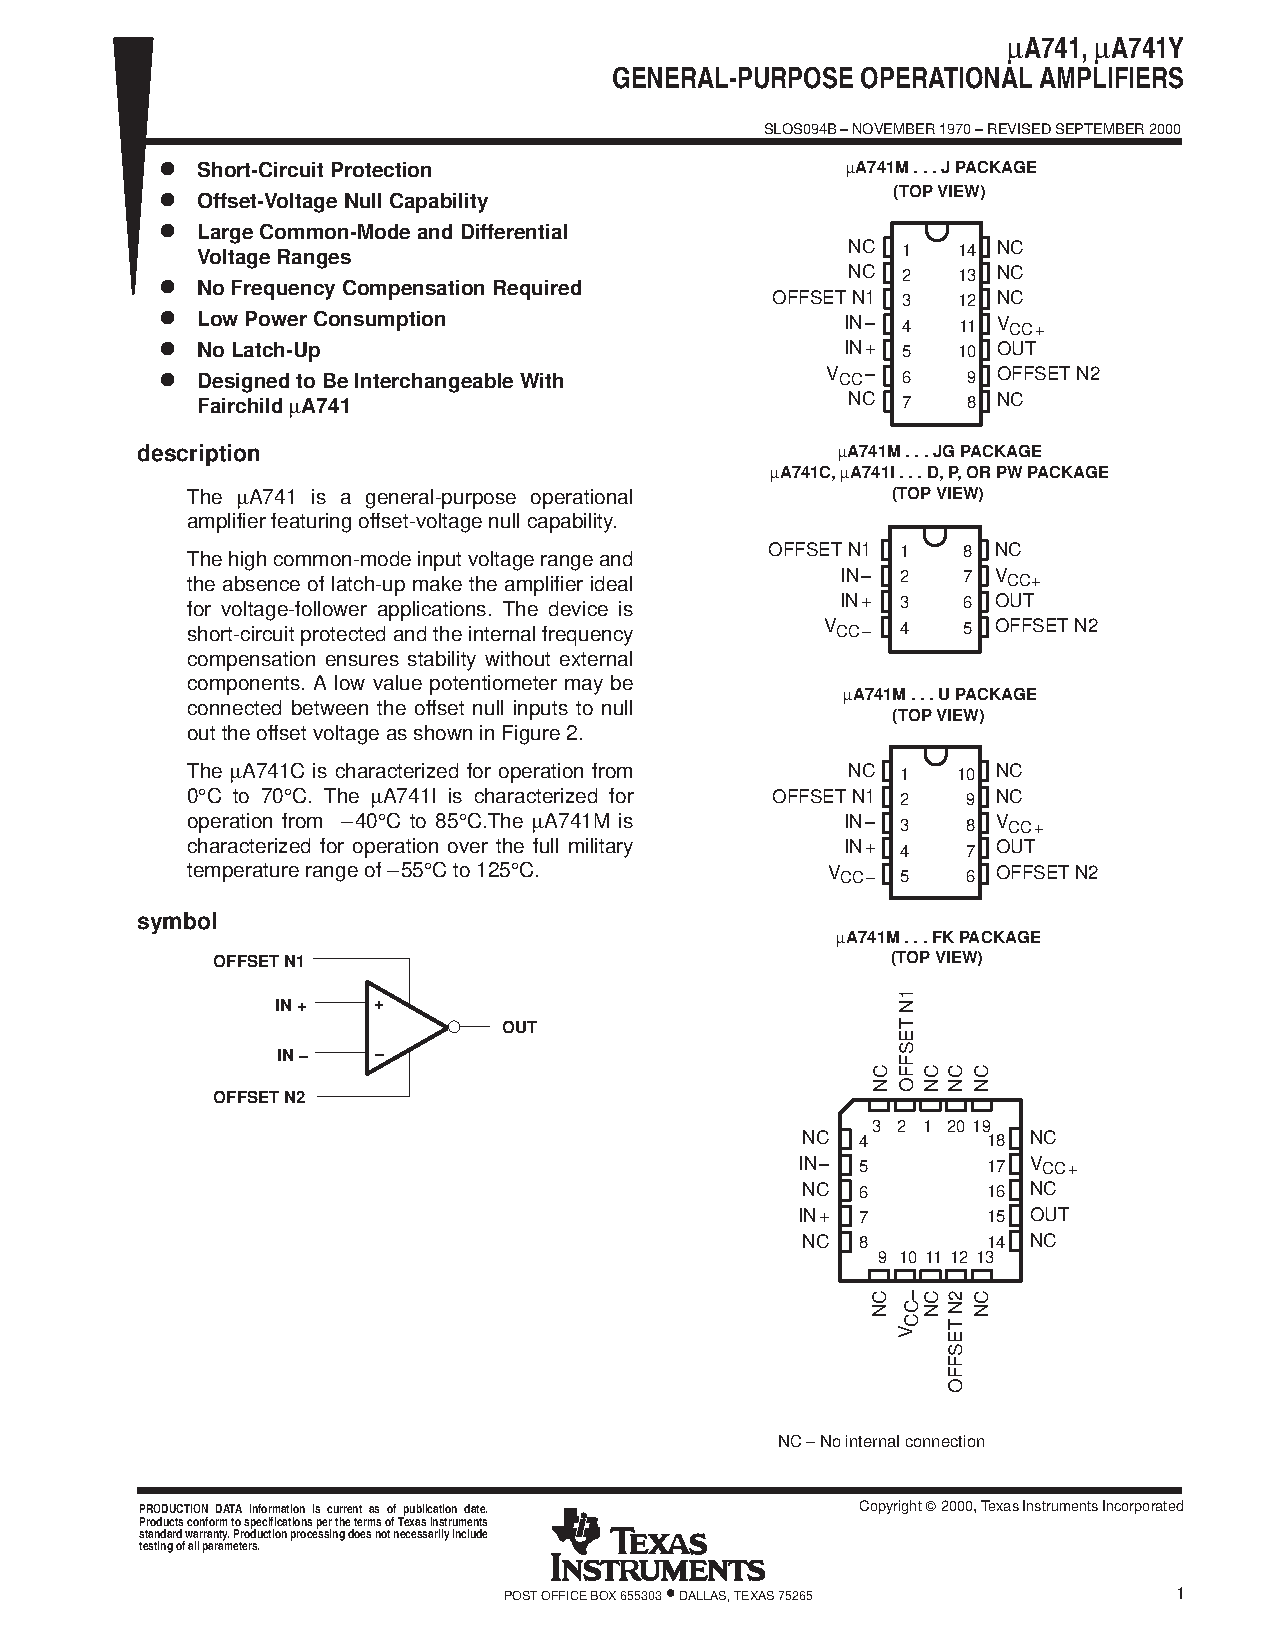
\includepdf[page=-, width=0.9\textwidth]{UA741MU.pdf}
\captionof{ilustracion}{Hoja de datos del amplificador operacional UA741MU}

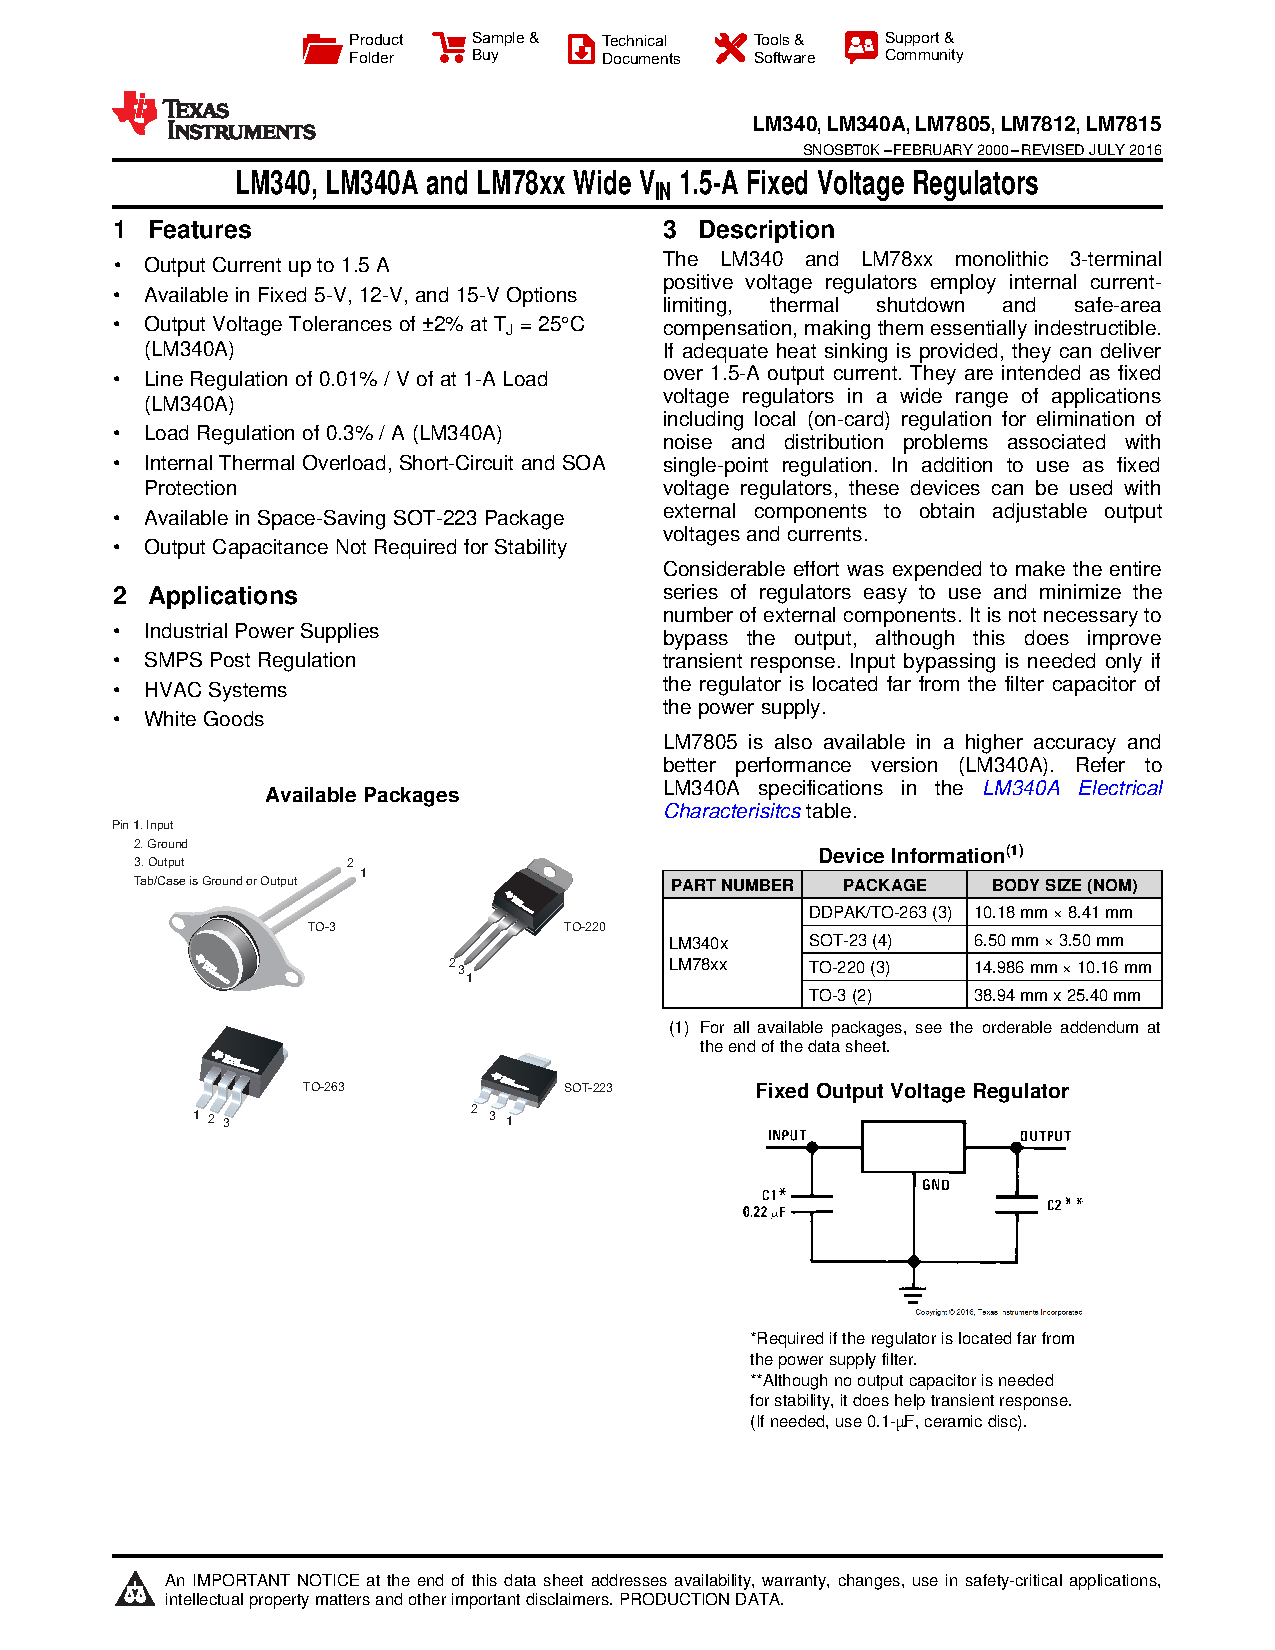
\includepdf[page=-, width=0.9\textwidth]{LM340.pdf}
\captionof{ilustracion}{Hoja de datos del LM340}

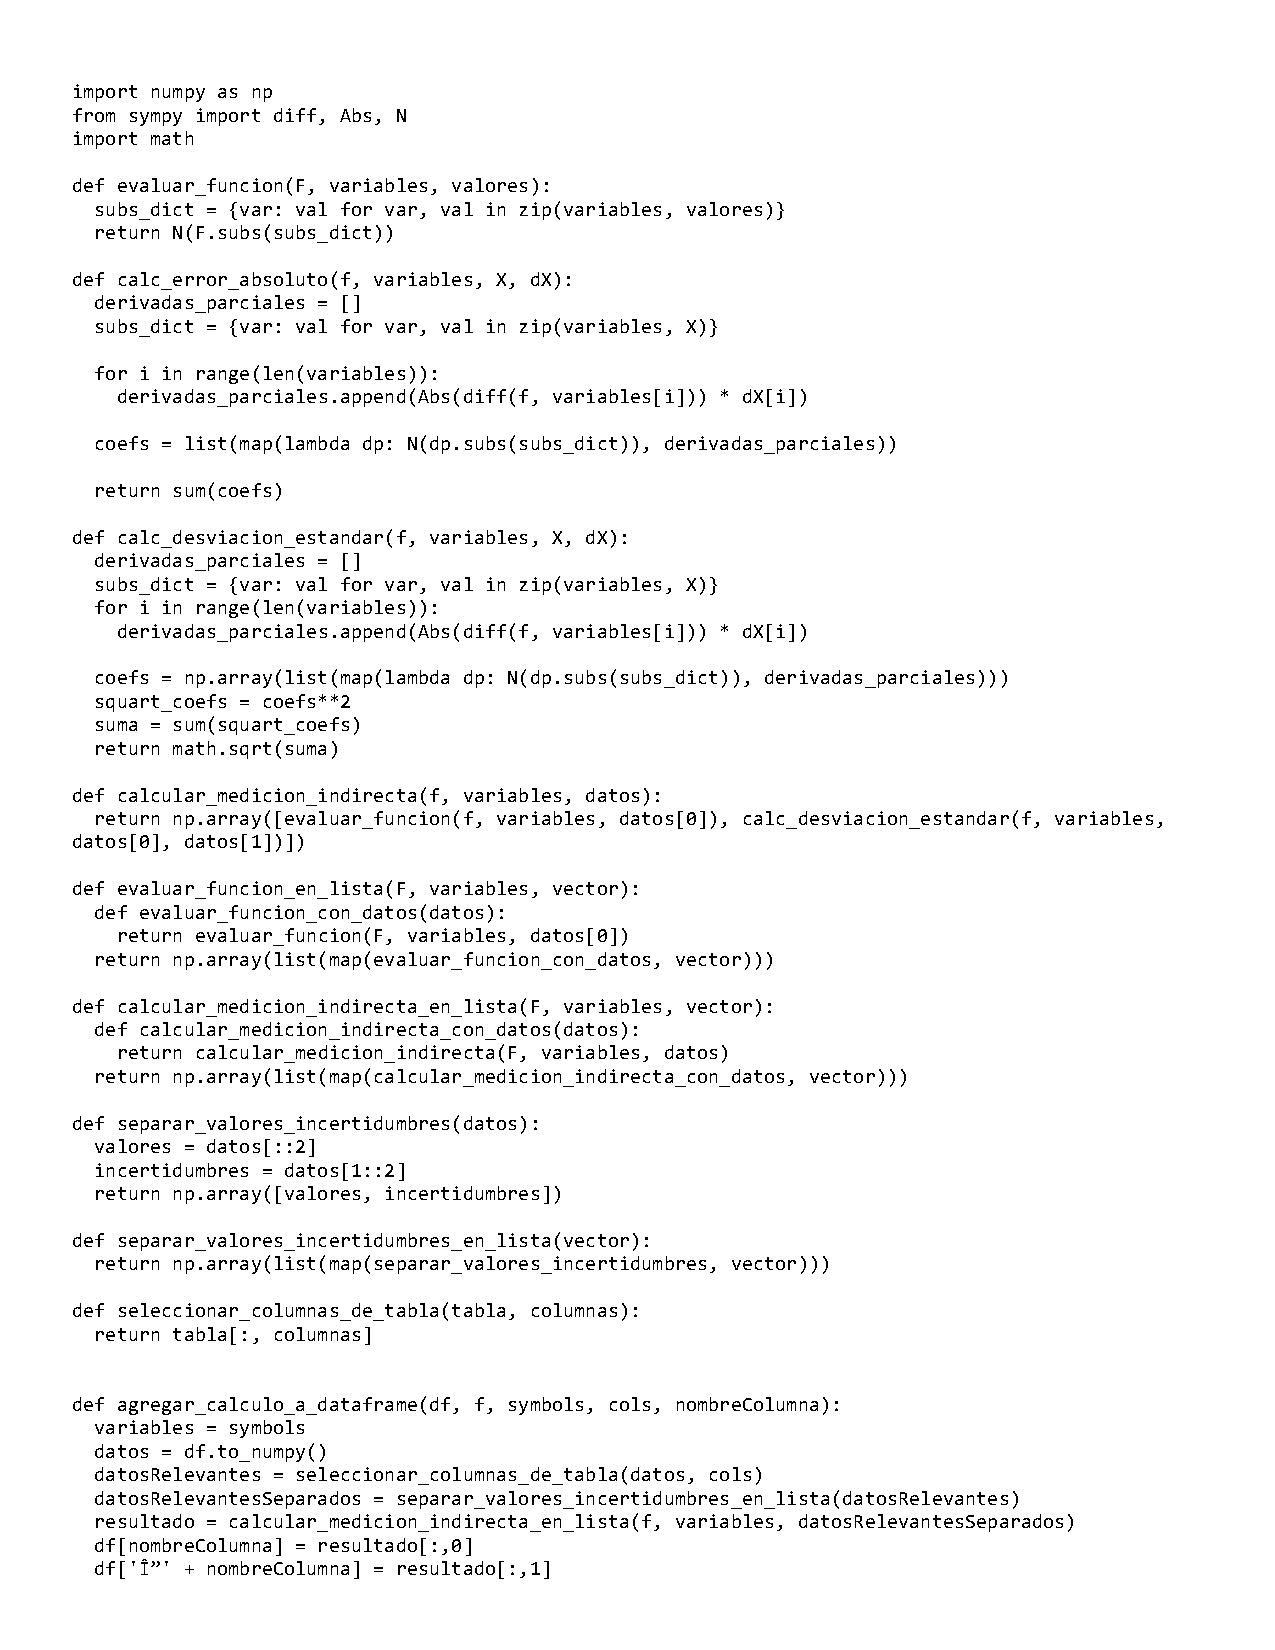
\includepdf[page=-, width=0.9\textwidth]{incertidumbres.pdf}
\captionof{ilustracion}{Código para calcular las mediciones indirectas y sus incertidumbres}

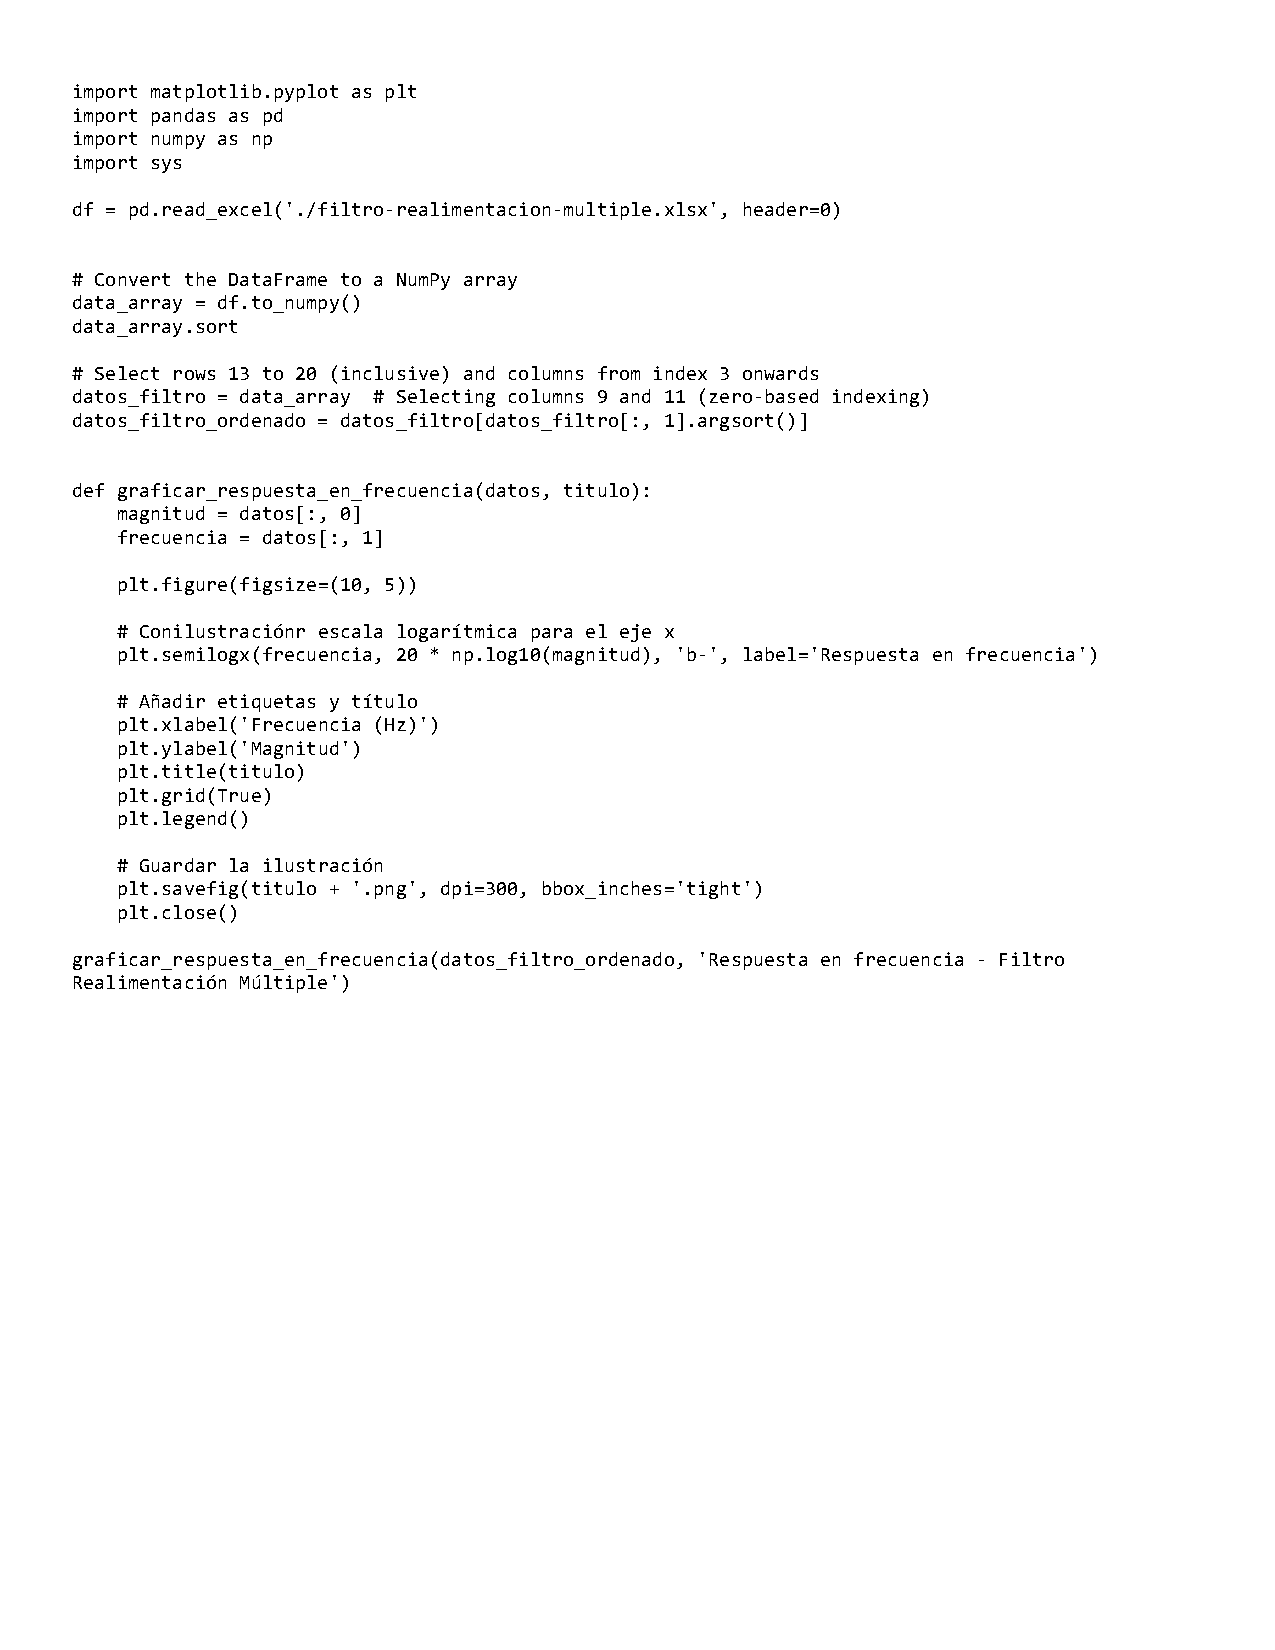
\includepdf[page=-, width=0.9\textwidth]{respuesta_en_frecuencia.pdf}
\captionof{ilustracion}{Código para graficar la respuesta en frecuencia}

